\documentclass[11pt,a4paper]{article}

% ── Packages ──────────────────────────────────────────────────────────
\usepackage[margin=1in]{geometry}
\usepackage{graphicx}
\usepackage{xcolor}
\usepackage{listings}
\usepackage{booktabs}
\usepackage{longtable}
\usepackage{array}
\usepackage{enumitem}
\usepackage{hyperref}
\usepackage{tikz}
\usepackage{fancyhdr}
\usepackage{titlesec}
\usepackage{float}
\usepackage{amsmath}
\usepackage{textcomp}

\usetikzlibrary{arrows.meta,positioning,shapes.geometric,fit,calc,decorations.pathreplacing}

% ── Colors ────────────────────────────────────────────────────────────
\definecolor{masterblue}{RGB}{41,98,255}
\definecolor{elecgreen}{RGB}{22,163,74}
\definecolor{pressorange}{RGB}{234,88,12}
\definecolor{servopurple}{RGB}{147,51,234}
\definecolor{codebg}{RGB}{248,248,248}
\definecolor{codeframe}{RGB}{200,200,200}
\definecolor{keywordblue}{RGB}{0,0,180}
\definecolor{commentgreen}{RGB}{0,128,0}
\definecolor{stringred}{RGB}{163,21,21}

% ── Listings Style ────────────────────────────────────────────────────
\lstdefinestyle{cppstyle}{
  language=C++,
  basicstyle=\ttfamily\small,
  backgroundcolor=\color{codebg},
  frame=single,
  rulecolor=\color{codeframe},
  keywordstyle=\color{keywordblue}\bfseries,
  commentstyle=\color{commentgreen}\itshape,
  stringstyle=\color{stringred},
  numbers=left,
  numberstyle=\tiny\color{gray},
  numbersep=8pt,
  breaklines=true,
  tabsize=2,
  showstringspaces=false,
  columns=flexible,
  morekeywords={uint8_t,uint16_t,uint32_t,int32_t,bool,QueueHandle_t,
    esp_err_t,TaskHandle_t,BaseType_t,TickType_t,pdTRUE,pdFALSE,
    WIFI_IF_AP,WIFI_IF_STA,ESP_OK}
}

% ── Header/Footer ────────────────────────────────────────────────────
\pagestyle{fancy}
\fancyhf{}
\fancyhead[L]{\small\textsc{AVCC Electronics}}
\fancyhead[R]{\small\textsc{System Architecture}}
\fancyfoot[C]{\thepage}
\renewcommand{\headrulewidth}{0.4pt}

% ── Section Formatting ───────────────────────────────────────────────
\titleformat{\section}{\Large\bfseries\color{masterblue}}{\thesection}{1em}{}
\titleformat{\subsection}{\large\bfseries}{\thesubsection}{1em}{}
\titleformat{\subsubsection}{\normalsize\bfseries}{\thesubsubsection}{1em}{}

% ── Hyperref ─────────────────────────────────────────────────────────
\hypersetup{
  colorlinks=true,
  linkcolor=masterblue,
  urlcolor=masterblue,
  citecolor=masterblue,
  pdftitle={AVCC Electronics System Architecture},
  pdfauthor={AVCC Team}
}

% ══════════════════════════════════════════════════════════════════════
\begin{document}

% ── Title Page ────────────────────────────────────────────────────────
\begin{titlepage}
\centering
\vspace*{2cm}
{\Huge\bfseries AVCC Electronics\\[0.3cm]System Architecture}\\[1.5cm]
{\Large\textsc{Detailed Technical Reference}}\\[2cm]
{\large
\begin{tabular}{rl}
\textbf{Platform:}    & ESP32 (Espressif, Arduino Core 2.0.14 / ESP-IDF 5.x) \\
\textbf{Protocol:}    & ESP-NOW (250\,kbps, 250\,byte max payload) \\
\textbf{Topology:}    & 1 Master + 3 Slaves (star) \\
\textbf{Channels:}    & 12 per slave (36 total outputs) \\
\end{tabular}
}\\[3cm]
\vfill
{\small Generated \today}
\end{titlepage}

\tableofcontents
\newpage

% ══════════════════════════════════════════════════════════════════════
\section{System Overview}
% ══════════════════════════════════════════════════════════════════════

The AVCC (Autonomous Vascular Compression Controller) Electronics system is a
real-time, wireless, multi-channel waveform controller built on four ESP32
microcontrollers connected via ESP-NOW. It drives three different output
modalities---analog voltage (electrical), digital solenoid (pressure), and
servo motor---synchronized from a single master controller.

\subsection{High-Level Topology}

\begin{center}
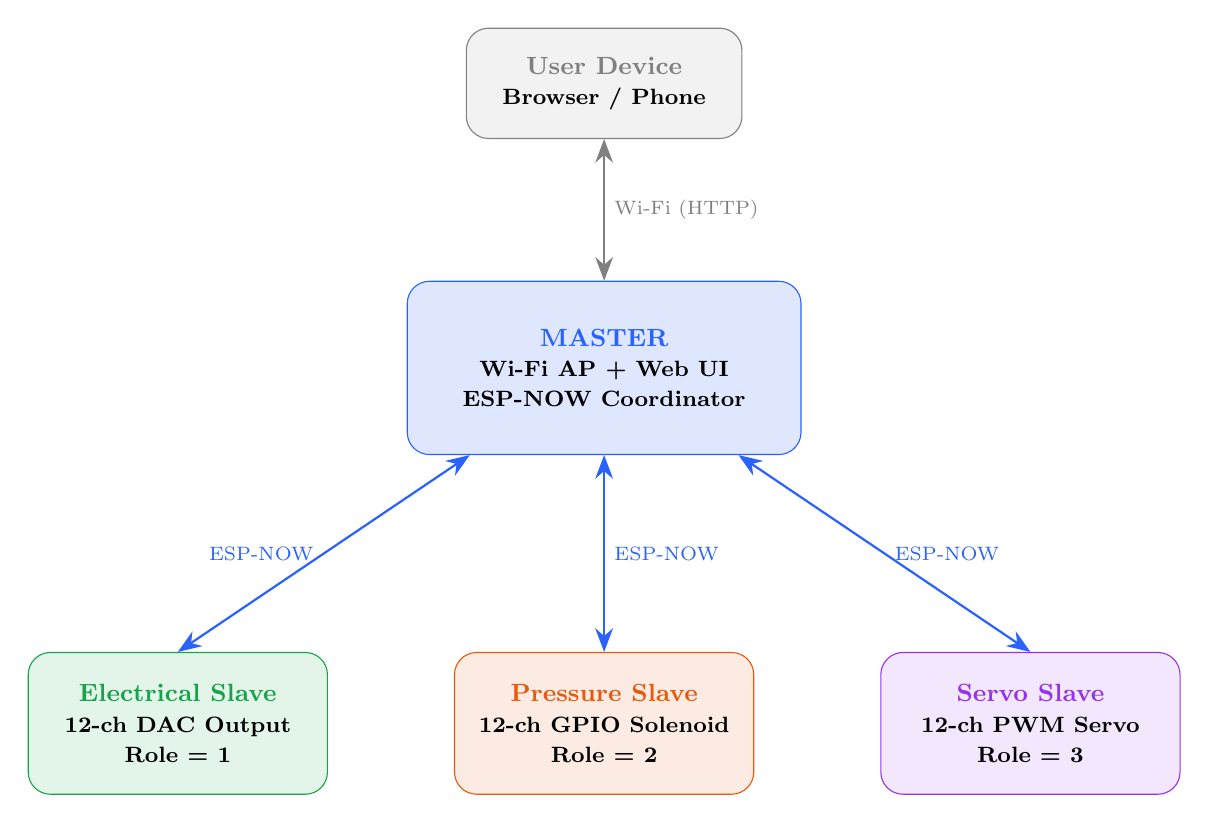
\begin{tikzpicture}[
  node distance=2.5cm,
  device/.style={rectangle, draw, rounded corners=8pt, minimum width=3.8cm, minimum height=1.8cm, align=center, font=\small\bfseries},
  link/.style={-{Stealth[length=3mm]}, thick},
  bilink/.style={{Stealth[length=3mm]}-{Stealth[length=3mm]}, thick},
]
  % Master
  \node[device, fill=masterblue!15, draw=masterblue, minimum width=5cm, minimum height=2.2cm] (master) {
    \textcolor{masterblue}{MASTER}\\
    \footnotesize Wi-Fi AP + Web UI\\
    \footnotesize ESP-NOW Coordinator
  };

  % Slaves
  \node[device, fill=elecgreen!12, draw=elecgreen, below left=2.5cm and 1cm of master] (elec) {
    \textcolor{elecgreen}{Electrical Slave}\\
    \footnotesize 12-ch DAC Output\\
    \footnotesize Role = 1
  };
  \node[device, fill=pressorange!12, draw=pressorange, below=2.5cm of master] (press) {
    \textcolor{pressorange}{Pressure Slave}\\
    \footnotesize 12-ch GPIO Solenoid\\
    \footnotesize Role = 2
  };
  \node[device, fill=servopurple!12, draw=servopurple, below right=2.5cm and 1cm of master] (servo) {
    \textcolor{servopurple}{Servo Slave}\\
    \footnotesize 12-ch PWM Servo\\
    \footnotesize Role = 3
  };

  % Links
  \draw[bilink, masterblue] (master.south west) ++(0.8,0) -- (elec.north) node[midway, left, font=\scriptsize] {ESP-NOW};
  \draw[bilink, masterblue] (master.south) -- (press.north) node[midway, right, font=\scriptsize] {ESP-NOW};
  \draw[bilink, masterblue] (master.south east) ++(-0.8,0) -- (servo.north) node[midway, right, font=\scriptsize] {ESP-NOW};

  % User
  \node[device, fill=gray!10, draw=gray, above=1.8cm of master, minimum width=3.5cm, minimum height=1.4cm] (user) {
    \textcolor{gray}{User Device}\\
    \footnotesize Browser / Phone
  };
  \draw[bilink, gray] (user.south) -- (master.north) node[midway, right, font=\scriptsize] {Wi-Fi (HTTP)};
\end{tikzpicture}
\end{center}

\subsection{Communication Flow Summary}

\begin{enumerate}[leftmargin=2cm]
  \item \textbf{User} connects to the Master's Wi-Fi AP (\texttt{AVCC\_Master 5}, password \texttt{12345678}) and opens \texttt{http://192.168.4.1}.
  \item \textbf{Master} serves a streamed HTML control page where the user configures 12 channels (frequency, pulse width, amplitude, pressure duration, phase offsets).
  \item On \textbf{Apply + Start}, the Master enters the \texttt{MS\_WAIT\_ACKS} state, burst-sends \texttt{CMD\_SET} messages for all 12 channels to all 3 slaves, followed by targeted \texttt{CMD\_START} messages.
  \item Each \textbf{Slave} receives messages via a FreeRTOS queue, applies per-channel configuration, and sends back \texttt{AckMsg} (0xA1) confirmations.
  \item During operation (\texttt{MS\_RUNNING}), the Master sends \texttt{CMD\_KEEPALIVE} at 6.7\,Hz. Slaves auto-stop if no keepalive arrives within 500\,ms.
  \item Slaves send \texttt{StatusMsg} (0xA2) at 1\,Hz with health telemetry (heap, heartbeat age, sequence watermark).
\end{enumerate}

% ══════════════════════════════════════════════════════════════════════
\section{Wire Protocol}
% ══════════════════════════════════════════════════════════════════════

All messages are sent as raw ESP-NOW payloads. Structs use
\texttt{\_\_attribute\_\_((packed))} to eliminate padding and guarantee
byte-exact layout across devices.

\subsection{Command Message (\texttt{Msg}) --- Master $\to$ Slaves}

\begin{center}
\begin{tabular}{llcl}
\toprule
\textbf{Field} & \textbf{Type} & \textbf{Offset} & \textbf{Description} \\
\midrule
\texttt{cmd}            & \texttt{uint8\_t}  & 0  & Command code (1--4) \\
\texttt{ch}             & \texttt{uint8\_t}  & 1  & Channel 1--12 (0 = all) \\
\texttt{flags}          & \texttt{uint8\_t}  & 2  & Bitfield (see below) \\
\texttt{neutral\_code}  & \texttt{uint8\_t}  & 3  & DAC neutral code (0x80) \\
\texttt{run\_id}        & \texttt{uint32\_t} & 4  & Monotonic run identifier \\
\texttt{seq}            & \texttt{uint32\_t} & 8  & Per-channel sequence number \\
\texttt{period\_us}     & \texttt{uint32\_t} & 12 & Full cycle period ($\mu$s) \\
\texttt{pulse\_us}      & \texttt{uint32\_t} & 16 & Pulse width ($\mu$s) \\
\texttt{pos\_code}      & \texttt{uint8\_t}  & 20 & Positive DAC code \\
\texttt{neg\_code}      & \texttt{uint8\_t}  & 21 & Negative DAC code \\
\texttt{rsv0}           & \texttt{uint8\_t}  & 22 & Reserved \\
\texttt{rsv1}           & \texttt{uint8\_t}  & 23 & Reserved \\
\texttt{start\_delay\_us}  & \texttt{uint32\_t} & 24 & Sync start delay ($\mu$s) \\
\texttt{phase\_offset\_us} & \texttt{uint32\_t} & 28 & Phase offset ($\mu$s) \\
\texttt{duration\_ms}      & \texttt{uint32\_t} & 32 & Run duration (ms); 0 = forever \\
\bottomrule
\end{tabular}
\end{center}

\textbf{Total size:} 36 bytes (V3). The legacy V1 format is 24 bytes (no \texttt{start\_delay\_us}, \texttt{phase\_offset\_us}, \texttt{duration\_ms}). Pressure and Servo slaves auto-detect V1 by checking \texttt{len == sizeof(MsgV1)}.

\subsubsection{Command Codes}

\begin{center}
\begin{tabular}{clp{8cm}}
\toprule
\textbf{Value} & \textbf{Name} & \textbf{Description} \\
\midrule
1 & \texttt{CMD\_SET}       & Configure channel parameters (period, pulse, amplitude). Does not start output. \\
2 & \texttt{CMD\_START}     & Begin waveform output. Carries start delay, phase offset, and duration. \\
3 & \texttt{CMD\_STOP}      & Immediately stop all channels and park outputs at safe state. \\
4 & \texttt{CMD\_KEEPALIVE} & Heartbeat ping. Resets each slave's failsafe timer. \\
\bottomrule
\end{tabular}
\end{center}

\subsubsection{Flag Bits}

\begin{center}
\begin{tabular}{cll}
\toprule
\textbf{Bit} & \textbf{Constant} & \textbf{Meaning} \\
\midrule
0 & \texttt{FLG\_SET\_MIRROR} (0x01) & Mirror waveform around neutral (electrical only) \\
1 & \texttt{FLG\_TGT\_ELEC}  (0x02) & START targets the Electrical slave \\
2 & \texttt{FLG\_TGT\_PRES}  (0x04) & START targets the Pressure slave \\
3 & \texttt{FLG\_TGT\_MOTO}  (0x08) & START targets the Servo slave \\
\bottomrule
\end{tabular}
\end{center}

\subsection{Acknowledgment Message (\texttt{AckMsg}) --- Slaves $\to$ Master}

\begin{center}
\begin{tabular}{llcl}
\toprule
\textbf{Field} & \textbf{Type} & \textbf{Offset} & \textbf{Description} \\
\midrule
\texttt{type}    & \texttt{uint8\_t}  & 0  & Always 0xA1 \\
\texttt{role}    & \texttt{uint8\_t}  & 1  & 1=Electrical, 2=Pressure, 3=Motor \\
\texttt{cmd}     & \texttt{uint8\_t}  & 2  & Echoed command code \\
\texttt{ch}      & \texttt{uint8\_t}  & 3  & Echoed channel (0 for STOP) \\
\texttt{run\_id} & \texttt{uint32\_t} & 4  & Echoed run ID \\
\texttt{seq}     & \texttt{uint32\_t} & 8  & Echoed sequence number \\
\texttt{ok}      & \texttt{uint8\_t}  & 12 & 1 = accepted, 0 = rejected \\
\texttt{rsv[3]}  & \texttt{uint8\_t}  & 13 & Reserved padding \\
\bottomrule
\end{tabular}
\end{center}

\textbf{Total size:} 16 bytes.

\subsection{Status Message (\texttt{StatusMsg}) --- Slaves $\to$ Master}

\begin{center}
\begin{tabular}{llcl}
\toprule
\textbf{Field} & \textbf{Type} & \textbf{Offset} & \textbf{Description} \\
\midrule
\texttt{type}          & \texttt{uint8\_t}  & 0  & Always 0xA2 \\
\texttt{role}          & \texttt{uint8\_t}  & 1  & Slave role identifier \\
\texttt{rsv0, rsv1}    & \texttt{uint8\_t}  & 2  & Reserved \\
\texttt{millis\_now}   & \texttt{uint32\_t} & 4  & Slave's \texttt{millis()} timestamp \\
\texttt{run\_id}       & \texttt{uint32\_t} & 8  & Current run ID on slave \\
\texttt{last\_seq\_max}& \texttt{uint32\_t} & 12 & Highest sequence number seen \\
\texttt{hb\_age\_ms}   & \texttt{uint16\_t} & 16 & Keepalive age (ms), capped at 65535 \\
\texttt{free\_heap}    & \texttt{uint16\_t} & 18 & Free heap (bytes), capped at 65535 \\
\bottomrule
\end{tabular}
\end{center}

\textbf{Total size:} 20 bytes. Sent at 1\,Hz by each slave.

\subsection{Sequence Guard Mechanism}

Each slave maintains a per-channel sequence counter \texttt{lastSeq[12]}. When a
\texttt{CMD\_SET} or \texttt{CMD\_START} arrives, the slave checks:

\begin{lstlisting}[style=cppstyle]
static inline bool acceptSeq(uint8_t idx0, const Msg &m) {
  if (m.seq <= lastSeq[idx0]) return false;  // stale -> reject
  lastSeq[idx0] = m.seq;
  if (m.seq > lastSeqMax) lastSeqMax = m.seq;
  return true;
}
\end{lstlisting}

When a new \texttt{run\_id} is detected (master restarted), all sequence
counters are reset to 0 so fresh commands are accepted.

% ══════════════════════════════════════════════════════════════════════
\section{Master Controller}
% ══════════════════════════════════════════════════════════════════════

\textbf{File:} \texttt{Master\_Pressure\_Servo\_Electrical.ino} (1049 lines)

\subsection{Wi-Fi and Web Server}

The Master runs in \texttt{WIFI\_AP} mode (not \texttt{AP\_STA}) to avoid radio
instability on ESP-IDF~5.x. It creates a soft access point:

\begin{center}
\begin{tabular}{ll}
\toprule
\textbf{Parameter} & \textbf{Value} \\
\midrule
SSID       & \texttt{AVCC\_Master 5} \\
Password   & \texttt{12345678} \\
Channel    & 1 \\
Max clients & 4 \\
IP address & \texttt{192.168.4.1} \\
\bottomrule
\end{tabular}
\end{center}

The web server uses \textbf{streamed HTML} (chunked transfer encoding) via
\texttt{server.sendContent()} to avoid heap-killing \texttt{String}
concatenation. All HTML is built with stack-allocated \texttt{char buf[]}
arrays and \texttt{snprintf()}.

\texttt{WEBSERVER\_MAX\_POST\_ARGS} is set to \textbf{100} (default 32) because
the form has $12 \times 7 = 84$ channel fields plus control buttons.

\subsubsection{HTTP Endpoints}

\begin{center}
\begin{tabular}{lll}
\toprule
\textbf{Method} & \textbf{Path} & \textbf{Handler} \\
\midrule
GET  & \texttt{/}             & \texttt{handleRoot()} -- serve control page \\
POST & \texttt{/apply}        & \texttt{handleApply()} -- apply/start/stop \\
POST & \texttt{/save}         & \texttt{handleSave()} -- save to NVS flash \\
POST & \texttt{/load}         & \texttt{handleLoad()} -- reload from NVS \\
POST & \texttt{/factory}      & \texttt{handleFactory()} -- factory defaults (RAM) \\
POST & \texttt{/factory\_save} & \texttt{handleFactorySave()} -- factory + save \\
GET  & \texttt{/favicon.ico}  & \texttt{handleFavicon()} -- 204 No Content \\
\bottomrule
\end{tabular}
\end{center}

\subsection{NVS Persistent Storage}

Settings are stored in the ESP32's Non-Volatile Storage (NVS) partition
under namespace \texttt{"avcc"}. Per-channel keys use a compact naming scheme:

\begin{center}
\begin{tabular}{lll}
\toprule
\textbf{Key pattern} & \textbf{Type} & \textbf{Content} \\
\midrule
\texttt{en\%02d} & Bool  & Channel enable \\
\texttt{f\%02d}  & Float & Frequency (Hz) \\
\texttt{pu\%02d} & UInt  & Pulse width ($\mu$s) \\
\texttt{a\%02d}  & Float & Amplitude (V) \\
\texttt{pd\%02d} & UInt  & Pressure duration (ms) \\
\texttt{pp\%02d} & UInt  & Pressure phase offset ($\mu$s) \\
\texttt{mp\%02d} & UInt  & Motor phase offset ($\mu$s) \\
\texttt{dbg}     & Bool  & Debug serial output \\
\texttt{boot}    & Bool  & Boot auto-start \\
\bottomrule
\end{tabular}
\end{center}

\subsection{Master State Machine}

The Master uses an explicit three-state machine to manage the apply/start/stop lifecycle:

\begin{center}
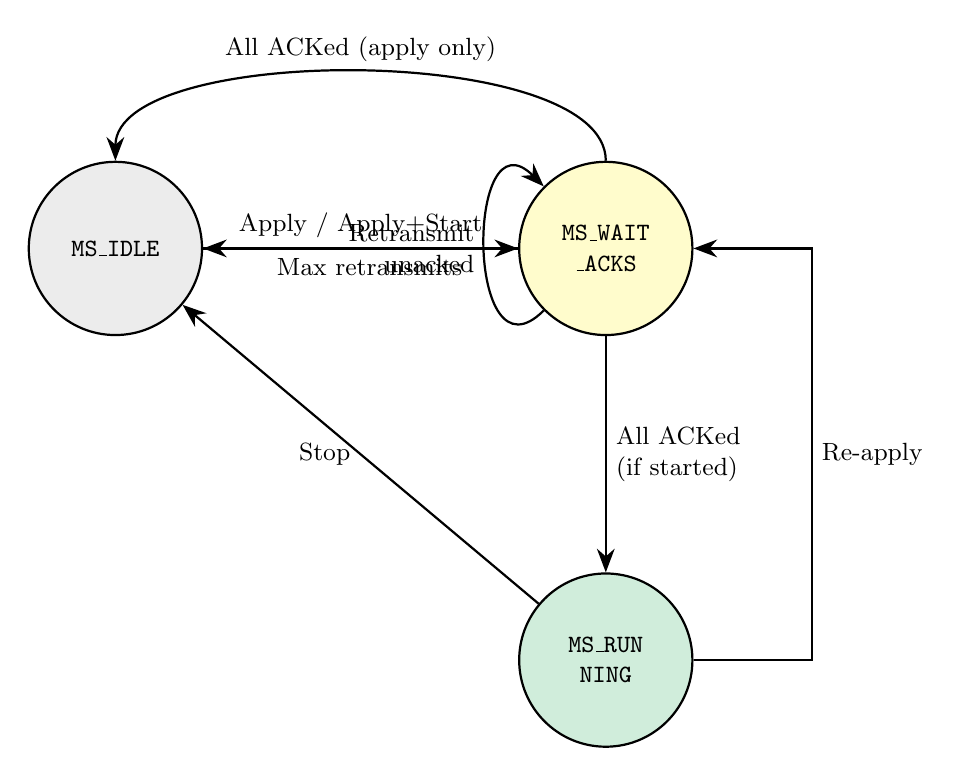
\begin{tikzpicture}[
  state/.style={circle, draw, thick, minimum size=2.2cm, align=center, font=\small\bfseries},
  trans/.style={-{Stealth[length=3mm]}, thick},
  every node/.style={font=\small},
]
  \node[state, fill=gray!15] (idle) {\texttt{MS\_IDLE}};
  \node[state, fill=yellow!20, right=4cm of idle] (wait) {\texttt{MS\_WAIT}\\\texttt{\_ACKS}};
  \node[state, fill=elecgreen!20, below=3cm of wait] (run) {\texttt{MS\_RUN}\\\texttt{NING}};

  % Transitions
  \draw[trans] (idle) -- (wait) node[midway, above] {Apply / Apply+Start};
  \draw[trans] (wait) -- (run) node[midway, right, align=left] {All ACKed\\(if started)};
  \draw[trans] (wait.north) .. controls +(0,1.5) and +(0,1.5) .. (idle.north) node[midway, above] {All ACKed (apply only)};
  \draw[trans] (wait) -- +(-2.5,0) |- (idle) node[near start, below, xshift=-0.5cm] {Max retransmits};
  \draw[trans] (run) -- (idle) node[midway, left] {Stop};
  \draw[trans] (run.east) -- +(1.5,0) |- (wait.east) node[near start, right] {Re-apply};

  % Self-loop on wait
  \draw[trans] (wait.south west) .. controls +(-1,-1) and +(-1,1) .. (wait.north west) node[midway, left, align=right] {Retransmit\\unacked};
\end{tikzpicture}
\end{center}

\begin{lstlisting}[style=cppstyle, caption={Master state types}]
enum MasterState : uint8_t {
  MS_IDLE,       // waiting for user input
  MS_WAIT_ACKS,  // sent SETs (and maybe STARTs), waiting for ACKs
  MS_RUNNING     // all channels active, sending keepalives
};

enum RequestType : uint8_t {
  REQ_APPLY_ONLY,  // send SETs only, return to IDLE
  REQ_APPLY_START,  // send SETs + STARTs, transition to RUNNING
  REQ_STOP          // send STOP, return to IDLE
};

struct PendingRequest {
  RequestType type;
  bool valid = false;
};
\end{lstlisting}

\subsection{Burst Send Architecture}

Instead of sending one channel per \texttt{loop()} iteration (the old
\texttt{applyOneStep()} pattern), the Master now sends all 12 channels in a
single burst:

\begin{enumerate}
  \item \textbf{\texttt{burstAllSets()}} --- Iterates over all 12 channels. For each enabled channel, increments its sequence number, constructs a \texttt{CMD\_SET} message, sends it to all 3 slaves via \texttt{sendSetToAll()}, and sets the corresponding bit in \texttt{unackedBitmap[3]}. Calls \texttt{yield()} after each channel to let the ESP-NOW TX queue drain.

  \item \textbf{\texttt{burstAllStarts()}} --- For each enabled channel, sends 3 targeted \texttt{CMD\_START} messages (one per slave) with appropriate \texttt{flags}, \texttt{phase\_offset\_us}, and \texttt{duration\_ms}. Each message gets a fresh sequence number.
\end{enumerate}

\subsection{Targeted Retransmission}

The Master tracks acknowledgments per-slave, per-channel:

\begin{lstlisting}[style=cppstyle]
struct SlaveHealth {
  uint32_t ackSeqCh[12];  // last acked seq per channel
  uint32_t expSeqCh[12];  // expected seq per channel
  // ...health telemetry...
};
SlaveHealth H[3];  // S_ELEC=0, S_PRES=1, S_MOTO=2
uint16_t unackedBitmap[3];  // per-slave bitmask of unacked channels
\end{lstlisting}

\texttt{retransmitUnacked()} only re-sends \texttt{CMD\_SET} messages to slaves
that haven't acknowledged specific channels, rather than broadcasting to all.
Up to \texttt{MAX\_RETRANSMITS} = 3 retries are attempted at 600\,ms intervals.

\subsection{Keepalive}

When \texttt{running == true}, the Master sends \texttt{CMD\_KEEPALIVE} to all
3 slaves every 150\,ms ($\approx$6.7\,Hz). This rate is deliberately lower
than the original 20\,Hz to reduce congestion with 3 slaves.

\subsection{Per-Channel Settings}

Each of the 12 channels has:

\begin{center}
\begin{tabular}{lll}
\toprule
\textbf{Parameter} & \textbf{Range} & \textbf{Default} \\
\midrule
Frequency (Hz)        & 0.01--10    & 0.5 \\
Pulse width ($\mu$s)  & 50--$T/2$  & 2000 \\
Amplitude (V)         & 0--15      & 15.0 \\
Pressure duration (ms) & 0+        & 330 \\
Pressure phase offset ($\mu$s) & 0+ & 0 \\
Motor phase offset ($\mu$s)    & 0+ & 0 \\
Enable                & bool       & true \\
\bottomrule
\end{tabular}
\end{center}

The amplitude is converted to an 8-bit DAC code using:
$$\texttt{code} = \text{round}\!\left(\frac{V + 15}{30} \times 255\right)$$
where $V \in [-15, +15]$ volts, giving code 0x00 for $-15$\,V and 0xFF for $+15$\,V, with 0x80 as the neutral midpoint.

% ══════════════════════════════════════════════════════════════════════
\section{Electrical Slave}
% ══════════════════════════════════════════════════════════════════════

\textbf{File:} \texttt{Electrical\_Receiver\_V2.ino} (755 lines)

This slave generates bipolar analog waveforms on 12 channels via an 8-bit
parallel DAC bus. It is the most architecturally complex slave due to its
dual-task design.

\subsection{Dual-Core Task Architecture}

\begin{center}
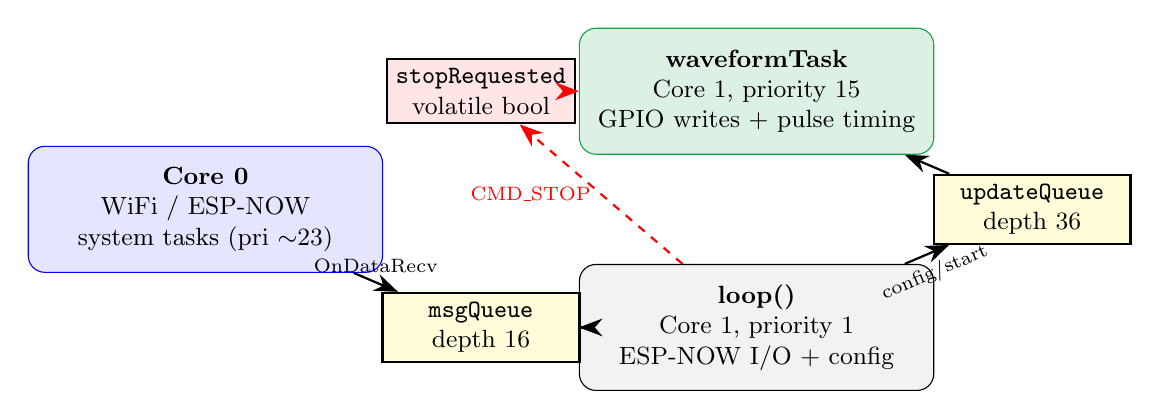
\begin{tikzpicture}[
  task/.style={rectangle, draw, rounded corners=6pt, minimum width=4.5cm, minimum height=1.6cm, align=center, font=\small},
  queue/.style={rectangle, draw, thick, fill=yellow!15, minimum width=2.5cm, minimum height=0.8cm, align=center, font=\small},
  arr/.style={-{Stealth[length=3mm]}, thick},
]
  % Core 0
  \node[task, fill=blue!10, draw=blue] (wifi) at (0,0) {\textbf{Core 0}\\WiFi / ESP-NOW\\system tasks (pri $\sim$23)};

  % Core 1
  \node[task, fill=elecgreen!15, draw=elecgreen] (wf) at (7,1.5) {\textbf{waveformTask}\\Core 1, priority 15\\GPIO writes + pulse timing};
  \node[task, fill=gray!10] (loop) at (7,-1.5) {\textbf{loop()}\\Core 1, priority 1\\ESP-NOW I/O + config};

  % Queues
  \node[queue] (msgq) at (3.5,-1.5) {\texttt{msgQueue}\\depth 16};
  \node[queue] (updq) at (10.5,0) {\texttt{updateQueue}\\depth 36};

  % Flag
  \node[rectangle, draw, thick, fill=red!10, minimum width=2cm, minimum height=0.6cm, align=center, font=\small] (stop) at (3.5,1.5) {\texttt{stopRequested}\\volatile bool};

  \draw[arr] (wifi) -- (msgq) node[midway, above, font=\scriptsize] {OnDataRecv};
  \draw[arr] (msgq) -- (loop);
  \draw[arr] (loop) -- (updq) node[midway, below, font=\scriptsize, sloped] {config/start};
  \draw[arr] (updq) -- (wf);
  \draw[arr, red, dashed] (loop) -- (stop) node[midway, left, font=\scriptsize] {CMD\_STOP};
  \draw[arr, red, dashed] (stop) -- (wf);
\end{tikzpicture}
\end{center}

\begin{itemize}
  \item \textbf{Core 0} runs WiFi and ESP-NOW system tasks at priority $\sim$23. The
    \texttt{OnDataRecv} callback executes here but \emph{only} enqueues packets
    into \texttt{msgQueue}---no processing.

  \item \textbf{Core 1} hosts two tasks:
    \begin{itemize}
      \item \texttt{waveformTask} (priority 15): owns all GPIO writes, the pulse
        scheduler, and the \texttt{ChanState[12]} array. Spin-waits when the
        next edge is $< 500\,\mu$s away for sub-millisecond timing precision.
      \item \texttt{loop()} (priority 1): handles all ESP-NOW I/O (receive,
        ACK, status), config parsing, and cross-task communication via
        \texttt{updateQueue}.
    \end{itemize}
\end{itemize}

\subsubsection{Adaptive Yield Strategy}

\texttt{waveformTask} dynamically adjusts its yield behavior based on
the time until the next scheduled edge:

\begin{center}
\begin{tabular}{lll}
\toprule
\textbf{Gap to next edge} & \textbf{Action} & \textbf{Rationale} \\
\midrule
$\leq 500\,\mu$s     & Spin-wait (no yield)  & Sub-ms critical window \\
500\,$\mu$s -- 2\,ms  & \texttt{taskYIELD()}  & Brief reschedule \\
2\,ms -- 5\,ms        & \texttt{vTaskDelay(1)} & One FreeRTOS tick \\
$> 5$\,ms             & \texttt{vTaskDelay(gap$-$2ms)} & Long sleep \\
No active channels    & \texttt{vTaskDelay(10)} & Deep idle \\
\bottomrule
\end{tabular}
\end{center}

\subsection{DAC Hardware Interface}

The Electrical slave drives 12 DAC channels through 3 quad-DAC chips
connected via an 8-bit parallel data bus:

\subsubsection{Pin Mapping}

\begin{center}
\begin{tabular}{lll}
\toprule
\textbf{Signal} & \textbf{GPIO(s)} & \textbf{Purpose} \\
\midrule
DB0--DB7  & 16, 15, 14, 13, 12, 5, 4, 2 & 8-bit data bus \\
DAC\_SEL0 & 17 & DAC channel select bit 0 \\
DAC\_SEL1 & 18 & DAC channel select bit 1 \\
WR1       & 23 & Write strobe, chip 1 (ch 1--4) \\
WR2       & 25 & Write strobe, chip 2 (ch 5--8) \\
WR3       & 26 & Write strobe, chip 3 (ch 9--12) \\
\bottomrule
\end{tabular}
\end{center}

\subsubsection{Write Sequence}

To set a channel's DAC output:

\begin{enumerate}
  \item Apply logical-to-physical channel remapping (swaps channels 2$\leftrightarrow$3, 6$\leftrightarrow$7, 10$\leftrightarrow$11).
  \item Write the 8-bit code to the data bus using direct GPIO register writes (\texttt{GPIO.out\_w1tc} / \texttt{GPIO.out\_w1ts}).
  \item Wait 1\,$\mu$s (data setup time).
  \item Set the DAC select lines (2-bit address within chip).
  \item Wait 1\,$\mu$s (select setup time).
  \item Strobe the appropriate WR pin LOW for 2\,$\mu$s, then HIGH (latch).
\end{enumerate}

Total write time: $\approx$4--5\,$\mu$s per channel update.

\subsection{Per-Channel State Machine}

Each electrical channel follows a 5-state machine for bipolar waveform generation:

\begin{center}
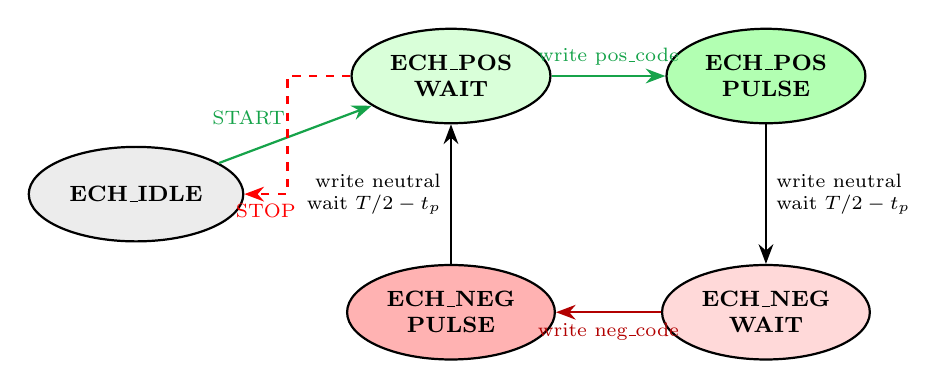
\begin{tikzpicture}[
  state/.style={ellipse, draw, thick, minimum width=2.4cm, minimum height=1.2cm, align=center, font=\footnotesize\bfseries},
  trans/.style={-{Stealth[length=2.5mm]}, thick},
]
  \node[state, fill=gray!15] (idle) at (0,0) {ECH\_IDLE};
  \node[state, fill=green!15] (pw) at (4,1.5) {ECH\_POS\\WAIT};
  \node[state, fill=green!30] (pp) at (8,1.5) {ECH\_POS\\PULSE};
  \node[state, fill=red!15] (nw) at (8,-1.5) {ECH\_NEG\\WAIT};
  \node[state, fill=red!30] (np) at (4,-1.5) {ECH\_NEG\\PULSE};

  \draw[trans, elecgreen] (idle) -- (pw) node[midway, above left, font=\scriptsize] {START};
  \draw[trans, elecgreen] (pw) -- (pp) node[midway, above, font=\scriptsize] {write pos\_code};
  \draw[trans] (pp) -- (nw) node[midway, right, font=\scriptsize, align=left] {write neutral\\wait $T/2 - t_p$};
  \draw[trans, red!70!black] (nw) -- (np) node[midway, below, font=\scriptsize] {write neg\_code};
  \draw[trans] (np) -- (pw) node[midway, left, font=\scriptsize, align=right] {write neutral\\wait $T/2 - t_p$};
  \draw[trans, red, dashed] (pw.west) -- ++(-0.8,0) |- (idle.east) node[near end, below, font=\scriptsize] {STOP};
\end{tikzpicture}
\end{center}

\begin{lstlisting}[style=cppstyle, caption={Electrical channel state enum}]
enum ElecChState : uint8_t {
  ECH_IDLE,       // channel disabled
  ECH_POS_WAIT,   // waiting for positive pulse edge
  ECH_POS_PULSE,  // positive pulse active (DAC = pos_code)
  ECH_NEG_WAIT,   // waiting for negative pulse edge
  ECH_NEG_PULSE   // negative pulse active (DAC = neg_code)
};
\end{lstlisting}

\textbf{Waveform timing (one full cycle):}
\begin{center}
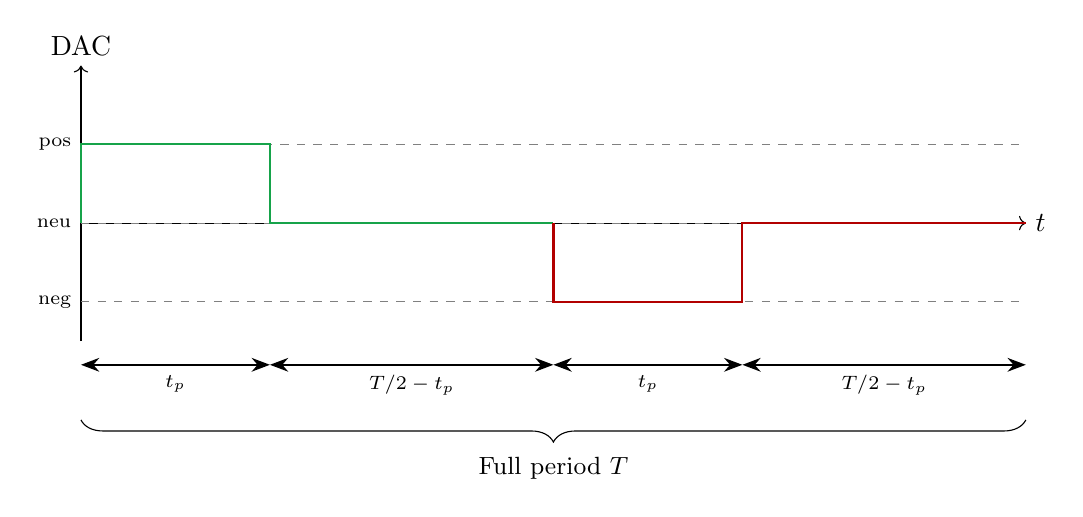
\begin{tikzpicture}[xscale=1.2]
  \draw[->] (0,0) -- (10,0) node[right] {$t$};
  \draw[->] (0,-1.5) -- (0,2) node[above] {DAC};

  % Labels
  \draw[dashed, gray] (0,1) -- (10,1);
  \node[left, font=\scriptsize] at (0,1) {pos};
  \draw[dashed, gray] (0,0) -- (10,0);
  \node[left, font=\scriptsize] at (0,0) {neu};
  \draw[dashed, gray] (0,-1) -- (10,-1);
  \node[left, font=\scriptsize] at (0,-1) {neg};

  % Positive half
  \draw[thick, elecgreen] (0,0) -- (0,1) -- (2,1) -- (2,0) -- (5,0);
  \draw[thick, red!70!black] (5,0) -- (5,-1) -- (7,-1) -- (7,0) -- (10,0);

  % Annotations
  \draw[{Stealth}-{Stealth}, thick] (0,-1.8) -- (2,-1.8) node[midway, below, font=\scriptsize] {$t_p$};
  \draw[{Stealth}-{Stealth}, thick] (2,-1.8) -- (5,-1.8) node[midway, below, font=\scriptsize] {$T/2 - t_p$};
  \draw[{Stealth}-{Stealth}, thick] (5,-1.8) -- (7,-1.8) node[midway, below, font=\scriptsize] {$t_p$};
  \draw[{Stealth}-{Stealth}, thick] (7,-1.8) -- (10,-1.8) node[midway, below, font=\scriptsize] {$T/2 - t_p$};
  \draw[decorate, decoration={brace, amplitude=8pt, mirror}] (0,-2.5) -- (10,-2.5) node[midway, below=10pt, font=\small] {Full period $T$};
\end{tikzpicture}
\end{center}

Where $t_p$ = \texttt{pulse\_us} and $T$ = \texttt{period\_us}.

\subsection{Inter-Task Communication}

\begin{center}
\begin{tabular}{lp{2.5cm}cp{5.5cm}}
\toprule
\textbf{Queue} & \textbf{Direction} & \textbf{Depth} & \textbf{Payload} \\
\midrule
\texttt{msgQueue} & ESP-NOW CB $\to$ \texttt{loop()} & 16 & \texttt{RxPacket}: 6-byte MAC + 36-byte \texttt{Msg} \\
\texttt{updateQueue} & \texttt{loop()} $\to$ \texttt{waveformTask} & 36 & \texttt{ChanUpdate}: type + channel config + nextEdge \\
\texttt{stopRequested} & \texttt{loop()} $\to$ \texttt{waveformTask} & 1 (flag) & \texttt{volatile bool} \\
\bottomrule
\end{tabular}
\end{center}

\subsection{Timing Constants}

\begin{center}
\begin{tabular}{llp{6cm}}
\toprule
\textbf{Constant} & \textbf{Value} & \textbf{Purpose} \\
\midrule
\texttt{MIN\_PULSE\_US}   & 50\,$\mu$s   & Minimum pulse width \\
\texttt{MIN\_PERIOD\_US}  & 100\,ms      & Maximum frequency (10\,Hz) \\
\texttt{MAX\_PERIOD\_US}  & 30\,s        & Minimum frequency (0.033\,Hz) \\
\texttt{HEARTBEAT\_TIMEOUT\_MS} & 500\,ms & Failsafe timeout \\
\texttt{STATUS\_PERIOD\_MS}     & 1000\,ms & Health report interval \\
\texttt{MAX\_EVENTS\_PER\_BURST} & 400    & Scheduler burst limit \\
\bottomrule
\end{tabular}
\end{center}

% ══════════════════════════════════════════════════════════════════════
\section{Pressure Slave}
% ══════════════════════════════════════════════════════════════════════

\textbf{File:} \texttt{Pressure\_Receiver\_V2.ino} (506 lines)

This slave controls 12 solenoid valves via digital GPIO outputs. It generates
a square wave by toggling each output HIGH/LOW at a rate of \textbf{two pulses
per full electrical period} (one pulse per half-cycle).

\subsection{GPIO Pin Mapping}

\begin{center}
\begin{tabular}{cccccccccccc}
\toprule
CH1 & CH2 & CH3 & CH4 & CH5 & CH6 & CH7 & CH8 & CH9 & CH10 & CH11 & CH12 \\
\midrule
19 & 14 & 15 & 23 & 25 & 26 & 0 & 2 & 4 & 5 & 12 & 13 \\
\bottomrule
\end{tabular}
\end{center}

\subsection{Per-Channel State Machine}

\begin{center}
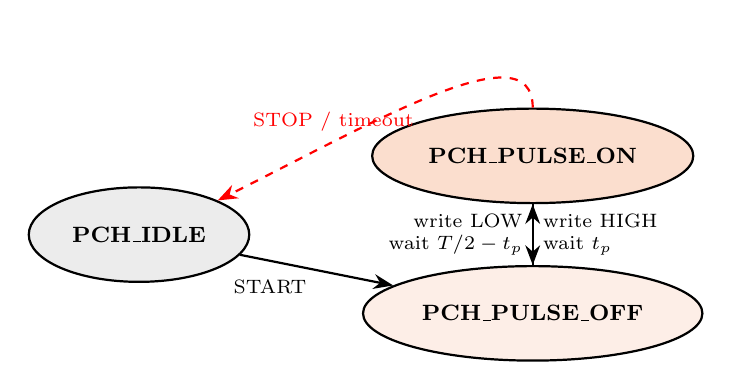
\begin{tikzpicture}[
  state/.style={ellipse, draw, thick, minimum width=2.8cm, minimum height=1.2cm, align=center, font=\footnotesize\bfseries},
  trans/.style={-{Stealth[length=2.5mm]}, thick},
]
  \node[state, fill=gray!15] (idle) at (0,0) {PCH\_IDLE};
  \node[state, fill=pressorange!20] (on) at (5,1) {PCH\_PULSE\_ON};
  \node[state, fill=pressorange!10] (off) at (5,-1) {PCH\_PULSE\_OFF};

  \draw[trans] (idle) -- (off) node[midway, below left, font=\scriptsize] {START};
  \draw[trans] (off) -- (on) node[midway, right, font=\scriptsize, align=left] {write HIGH\\wait $t_p$};
  \draw[trans] (on) -- (off) node[midway, left, font=\scriptsize, align=right] {write LOW\\wait $T/2 - t_p$};
  \draw[trans, red, dashed] (on.north) .. controls +(0,1) and +(2,1) .. (idle.north east) node[near end, above, font=\scriptsize] {STOP / timeout};
\end{tikzpicture}
\end{center}

\begin{lstlisting}[style=cppstyle, caption={Pressure channel state enum}]
enum PressChState : uint8_t {
  PCH_IDLE,       // disabled or not started
  PCH_PULSE_ON,   // output HIGH (pulse active)
  PCH_PULSE_OFF   // output LOW (off-portion of half-cycle)
};
\end{lstlisting}

\subsection{Duration Auto-Stop}

Each channel has a \texttt{stopAt\_ms} field. When \texttt{duration\_ms} is
non-zero in the \texttt{CMD\_START} message, the slave computes
\texttt{stopAt\_ms = millis() + duration\_ms}. Each \texttt{loop()} iteration
checks for expired channels:

\begin{lstlisting}[style=cppstyle]
if (chs[i].chState != PCH_IDLE &&
    chs[i].stopAt_ms != 0 &&
    (int32_t)(nowms - chs[i].stopAt_ms) >= 0) {
  chs[i].chState = PCH_IDLE;
  writePressure(i+1, false);
}
\end{lstlisting}

\subsection{FreeRTOS Message Queue}

The Pressure slave uses a FreeRTOS queue (depth 16) to safely pass messages from
the ESP-NOW receive callback to the main loop, preventing packet drops during
the Master's burst send of 12 channels:

\begin{lstlisting}[style=cppstyle]
struct RxPacket { uint8_t mac[6]; Msg msg; };
static QueueHandle_t msgQueue = nullptr;
static const int MSG_QUEUE_DEPTH = 16;
\end{lstlisting}

The callback (\texttt{OnDataRecv}) also supports backward-compatible V1 messages
by detecting \texttt{len == sizeof(MsgV1)} and zero-filling the V3 extension fields.

\subsection{Architecture Differences from Electrical}

\begin{center}
\begin{tabular}{lll}
\toprule
\textbf{Aspect} & \textbf{Electrical} & \textbf{Pressure} \\
\midrule
Threading    & Dual-task (waveformTask + loop) & Single-task (loop only) \\
Output       & 8-bit DAC (analog)              & Digital GPIO (HIGH/LOW) \\
Pulses/cycle & 2 (bipolar: pos + neg)          & 2 (both HIGH) \\
Stop method  & \texttt{stopRequested} flag      & Direct \texttt{safeStopAll()} \\
Duration     & Not supported                    & Per-channel auto-stop \\
\bottomrule
\end{tabular}
\end{center}

% ══════════════════════════════════════════════════════════════════════
\section{Servo Slave}
% ══════════════════════════════════════════════════════════════════════

\textbf{File:} \texttt{Servo\_Receiver\_V2.ino} (494 lines)

This slave drives 12 hobby servo motors with a ramp-up/ramp-down motion
profile. It has a 2\,Hz hard frequency cap to protect the mechanical servos.

\subsection{GPIO Pin Mapping}

Same physical pins as the Pressure slave:

\begin{center}
\begin{tabular}{cccccccccccc}
\toprule
CH1 & CH2 & CH3 & CH4 & CH5 & CH6 & CH7 & CH8 & CH9 & CH10 & CH11 & CH12 \\
\midrule
19 & 14 & 15 & 23 & 25 & 26 & 0 & 2 & 4 & 5 & 12 & 13 \\
\bottomrule
\end{tabular}
\end{center}

\subsection{Motion Profile}

\begin{center}
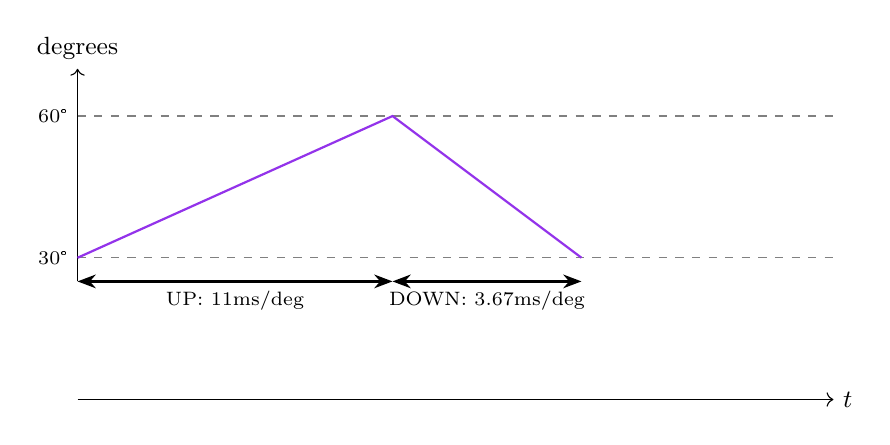
\begin{tikzpicture}[xscale=0.8, yscale=0.06]
  \draw[->] (0,0) -- (12,0) node[right, font=\small] {$t$};
  \draw[->] (0,25) -- (0,70) node[above, font=\small] {degrees};

  % DEG_MIN / DEG_MAX lines
  \draw[dashed, gray] (0,30) -- (12,30);
  \node[left, font=\scriptsize] at (0,30) {30\textdegree};
  \draw[dashed, gray] (0,60) -- (12,60);
  \node[left, font=\scriptsize] at (0,60) {60\textdegree};

  % Ramp up (slow) then ramp down (fast)
  \draw[thick, servopurple] (0,30) -- (5,60) -- (8,30) -- (8,30);

  % Annotations
  \draw[{Stealth}-{Stealth}, thick] (0,25) -- (5,25);
  \node[below, font=\scriptsize] at (2.5,25) {UP: 11ms/deg};
  \draw[{Stealth}-{Stealth}, thick] (5,25) -- (8,25);
  \node[below, font=\scriptsize] at (6.5,25) {DOWN: 3.67ms/deg};
\end{tikzpicture}
\end{center}

\begin{center}
\begin{tabular}{lll}
\toprule
\textbf{Parameter} & \textbf{Value} & \textbf{Description} \\
\midrule
\texttt{DEG\_MIN}     & 30\textdegree & Motion start/end angle \\
\texttt{DEG\_MAX}     & 60\textdegree & Motion peak angle \\
\texttt{UP\_STEP\_US}   & 11\,000\,$\mu$s & Time per degree during ramp-up \\
\texttt{DOWN\_STEP\_US} & 3\,667\,$\mu$s  & Time per degree during ramp-down \\
Range                 & 30\textdegree & Total sweep = 30 degrees \\
Up time               & $\sim$330\,ms  & $30 \times 11\,\text{ms}$ \\
Down time             & $\sim$110\,ms  & $30 \times 3.67\,\text{ms}$ \\
\bottomrule
\end{tabular}
\end{center}

\subsection{Per-Channel State Machine}

\begin{center}
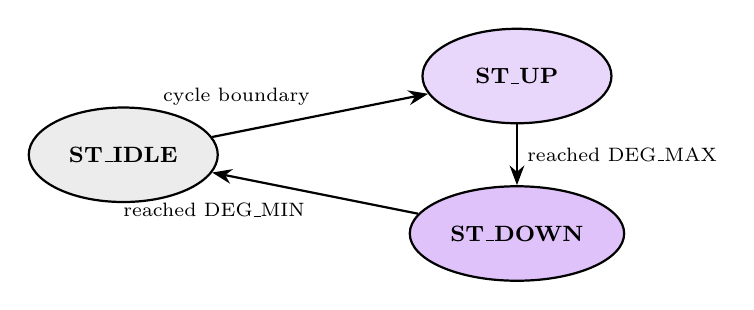
\begin{tikzpicture}[
  state/.style={ellipse, draw, thick, minimum width=2.4cm, minimum height=1.2cm, align=center, font=\footnotesize\bfseries},
  trans/.style={-{Stealth[length=2.5mm]}, thick},
]
  \node[state, fill=gray!15] (idle) at (0,0) {ST\_IDLE};
  \node[state, fill=servopurple!20] (up) at (5,1) {ST\_UP};
  \node[state, fill=servopurple!30] (down) at (5,-1) {ST\_DOWN};

  \draw[trans] (idle) -- (up) node[midway, above left, font=\scriptsize] {cycle boundary};
  \draw[trans] (up) -- (down) node[midway, right, font=\scriptsize] {reached DEG\_MAX};
  \draw[trans] (down) -- (idle) node[midway, below left, font=\scriptsize] {reached DEG\_MIN};
\end{tikzpicture}
\end{center}

The servo uses the existing \texttt{MotionStage} enum (unchanged from the original design):

\begin{lstlisting}[style=cppstyle]
enum MotionStage : uint8_t {
  ST_IDLE = 0,
  ST_UP   = 1,
  ST_DOWN = 2
};
\end{lstlisting}

\subsection{2\,Hz Hard Cap}

If the configured frequency exceeds 2\,Hz (\texttt{period\_us < 500000}), the
channel is disabled and the \texttt{CMD\_START} ACK is sent with
\texttt{ok = 0} (rejected). This protects the servo mechanism from being driven
faster than it can physically respond.

\subsection{Cycle Boundary Logic}

Unlike the Electrical and Pressure slaves which schedule edge events via
\texttt{nextEdge\_us}, the Servo slave uses a two-level scheduler:

\begin{enumerate}
  \item \textbf{Cycle boundary}: Each channel has a \texttt{nextCycle\_us} timestamp.
    When the current time passes this boundary, a new motion cycle is triggered
    (if the channel is idle) by calling \texttt{startMotion()}.
  \item \textbf{Step scheduler}: Within a motion cycle, each channel has a
    \texttt{nextStep\_us} timestamp. The servo angle is incremented/decremented
    by 1\textdegree{} at each step event.
\end{enumerate}

% ══════════════════════════════════════════════════════════════════════
\section{Synchronization and Timing}
% ══════════════════════════════════════════════════════════════════════

\subsection{Start Delay and Phase Offset}

When the Master sends \texttt{CMD\_START}, each slave computes its first edge as:

$$\texttt{nextEdge\_us} = \texttt{micros()} + \texttt{start\_delay\_us} + \texttt{phase\_offset\_us}$$

\begin{itemize}
  \item \texttt{start\_delay\_us} is a global constant (600\,ms default) that gives
    all slaves time to receive and process their START messages before any
    output begins.
  \item \texttt{phase\_offset\_us} is per-channel, per-slave, allowing the user
    to shift pressure and motor outputs relative to the electrical waveform.
\end{itemize}

\subsection{Keepalive Failsafe}

All 3 slaves implement the same heartbeat failsafe:

\begin{center}
\begin{tabular}{ll}
\toprule
\textbf{Parameter} & \textbf{Value} \\
\midrule
Master send rate & Every 150\,ms ($\sim$6.7\,Hz) \\
Slave timeout    & 500\,ms ($\sim$3 missed keepalives) \\
Action on timeout & \texttt{safeStopAll()} --- all outputs to safe state \\
\bottomrule
\end{tabular}
\end{center}

\textbf{Implementation difference:} The Electrical slave cannot call
\texttt{safeStopAll()} directly from \texttt{loop()} because that function
writes to GPIOs owned by \texttt{waveformTask} on the same core at
priority~15. Instead, it sets \texttt{stopRequested = true} and the waveform
task checks this flag at the top of each iteration. Pressure and Servo slaves
are single-threaded, so they call \texttt{safeStopAll()} directly.

\subsection{Peer Management}

\textbf{Master (AP mode):} Adds all 3 slave MACs as peers at startup using
\texttt{WIFI\_IF\_AP} interface. Channel is set to 0 (use current).

\textbf{Slaves (STA mode):} Dynamically add the Master as a peer when they
receive the first packet. The Master's MAC is extracted from the
\texttt{esp\_now\_recv\_info\_t} in the receive callback. A send-failure backoff
mechanism re-registers the peer after 3 consecutive \texttt{esp\_now\_send}
failures:

\begin{lstlisting}[style=cppstyle]
static inline void trackSendResult(esp_err_t e) {
  if (e == ESP_OK) { sendFailCount = 0; }
  else { if (++sendFailCount >= 3) masterPeerAdded = false; }
}
\end{lstlisting}

% ══════════════════════════════════════════════════════════════════════
\section{Safety Mechanisms}
% ══════════════════════════════════════════════════════════════════════

\subsection{Failsafe Summary}

\begin{center}
\begin{tabular}{p{4cm}p{8cm}}
\toprule
\textbf{Mechanism} & \textbf{Description} \\
\midrule
Heartbeat timeout & 500\,ms without keepalive $\to$ all outputs to safe state \\
Sequence guard & Per-channel monotonic sequence rejects stale/duplicate packets \\
Run ID reset & New \texttt{run\_id} resets all sequence counters to accept fresh commands \\
Timing guardrails & Period clamped to [100\,ms, 30\,s]; pulse clamped to [50\,$\mu$s, $T/2$] \\
Servo hard cap & Frequencies $> 2$\,Hz rejected; channel disabled \\
Peer re-registration & 3 send failures $\to$ peer deleted and re-added \\
Duration auto-stop & Pressure channels auto-stop after configured duration \\
Event burst limit & Max 400 events per scheduler iteration (prevents infinite loops) \\
\bottomrule
\end{tabular}
\end{center}

\subsection{Safe Stop Behavior}

\begin{center}
\begin{tabular}{ll}
\toprule
\textbf{Slave} & \textbf{Safe stop action} \\
\midrule
Electrical & All 12 DAC channels set to \texttt{neutral\_code} (0x80 = 0\,V) \\
Pressure   & All 12 GPIO outputs set LOW (solenoids off) \\
Servo      & All 12 servos driven to DEG\_MIN (30\textdegree{}) \\
\bottomrule
\end{tabular}
\end{center}

% ══════════════════════════════════════════════════════════════════════
\section{Memory and Performance}
% ══════════════════════════════════════════════════════════════════════

\subsection{Web Server Heap Management}

The Master's web UI avoids dynamic \texttt{String} allocation entirely. All
HTML is generated using stack-allocated \texttt{char buf[]} arrays with
\texttt{snprintf()} and streamed via \texttt{server.sendContent()}. The
\texttt{Connection: close} header and explicit \texttt{server.client().stop()}
ensure TCP sockets are released promptly.

The master dashboard displays real-time heap metrics (\texttt{ESP.getFreeHeap()}
and \texttt{ESP.getMaxAllocHeap()}) for monitoring memory health.

\subsection{Queue Sizing}

\begin{center}
\begin{tabular}{lccl}
\toprule
\textbf{Queue} & \textbf{Depth} & \textbf{Item size} & \textbf{Device} \\
\midrule
\texttt{msgQueue} (Electrical)  & 16 & 42\,B & Electrical slave \\
\texttt{updateQueue}            & 36 & $\sim$28\,B & Electrical slave \\
\texttt{msgQueue} (Pressure)    & 16 & 42\,B & Pressure slave \\
\texttt{msgQueue} (Servo)       & 16 & 42\,B & Servo slave \\
\bottomrule
\end{tabular}
\end{center}

The queue depth of 16 accommodates the Master's burst of 12 \texttt{CMD\_SET}
messages (one per channel) plus headroom for keepalives arriving during
processing. The Electrical slave's \texttt{updateQueue} has depth 36
($12 \times 3$) to hold 12 CONFIG + 12 START updates plus 12 spare.

% ══════════════════════════════════════════════════════════════════════
\section{Utility Sketches}
% ══════════════════════════════════════════════════════════════════════

\subsection{BICEP\_MAC\_Address}

A simple utility sketch that prints the ESP32's MAC address to Serial at
300\,baud. Used during initial hardware provisioning to discover each board's
MAC address for the Master's peer table.

\begin{lstlisting}[style=cppstyle]
void setup(){
  Serial.begin(300);
  Serial.print("ESP Board MAC Address:  ");
  Serial.println(WiFi.macAddress());
}
\end{lstlisting}

\subsection{Test\_on\_Wifi}

A diagnostic sketch that creates a Wi-Fi AP and confirms the ESP32's radio
is functional. Used for hardware bring-up testing.

% ══════════════════════════════════════════════════════════════════════
\section{Complete File Reference}
% ══════════════════════════════════════════════════════════════════════

\begin{center}
\begin{longtable}{p{6cm}cp{5.5cm}}
\toprule
\textbf{File} & \textbf{Lines} & \textbf{Role} \\
\midrule
\endhead
\texttt{Master\_Pressure\_Servo\_Electrical.ino} & 1049 & Central controller: Wi-Fi AP, Web UI, ESP-NOW coordinator, state machine \\
\texttt{Electrical\_Receiver\_V2.ino} & 755 & Electrical slave: 12-ch DAC output, dual-task architecture, sub-ms timing \\
\texttt{Pressure\_Receiver\_V2.ino} & 506 & Pressure slave: 12-ch GPIO solenoid control, duration auto-stop \\
\texttt{Servo\_Receiver\_V2.ino} & 494 & Servo slave: 12-ch servo motor, ramp profile, 2\,Hz hard cap \\
\texttt{BICEP\_MAC\_Address.ino} & 16 & Utility: print ESP32 MAC address \\
\texttt{Test\_on\_Wifi.ino} & --- & Utility: Wi-Fi AP smoke test \\
\bottomrule
\end{longtable}
\end{center}

% ══════════════════════════════════════════════════════════════════════
\section{Appendix: MAC Addresses (Current Configuration)}
% ══════════════════════════════════════════════════════════════════════

\begin{center}
\begin{tabular}{lll}
\toprule
\textbf{Device} & \textbf{MAC Address} & \textbf{Variable} \\
\midrule
Electrical slave & \texttt{94:54:C5:74:AB:38} & \texttt{mac\_elec[]} \\
Pressure slave   & \texttt{68:FE:71:0C:B9:50} & \texttt{mac\_press[]} \\
Servo slave      & \texttt{68:FE:71:0C:B7:F8} & \texttt{mac\_motor[]} \\
\bottomrule
\end{tabular}
\end{center}

\end{document}
